\chapter{Naive Mengenlehre}

\paragraph{Mengen} Zusammenfassung versch. Objekte ,,Elemente``.
\index{Menge}

\begin{description}
  \item[Element $x \mzSymbolEmph{\in} M$]
    \index{Element}
    ,,enthält``

  \item[Leere M. $\mzMathEmph{\emptyset}$]
    \index{Leere Menge}
    $=\{\}$

  \item[Universum $U$]
    \index{Universum}

  \item[Einschränkung]
    \index{Einschränkung}
    $\{ x \mid F(x) \}$
\end{description}

\subsection{Relationen}

\begin{description}
  \item[Teilmenge $N \subseteq M$]
    \index{Teilmenge}
    $\linebreak\Leftrightarrow \forall n \in N: n \in M$
    \mzInline{
      \begin{tikzpicture}[scale=.25]
        \filldraw[fill=white]
        (0,0) circle (4)
        node[right=8] {$M$};
        \filldraw[fill=background]
        (-1,0) circle (2)
        node {$N$};
      \end{tikzpicture}
    }

  \item[Gleichheit $M = N$]
    \index{Mengengleichheit}
    $\linebreak\Leftrightarrow M \subseteq N \land N \subseteq M$
    \mzInline{
      \begin{tikzpicture}[scale=.25]
        \filldraw[fill=background]
        (0,0) circle (2)
        node[above left=8] {$M$}
        node[above right=8] {$N$};
      \end{tikzpicture}
    }
\end{description}

\subsection{Mächtigkeit}
\index{Mächtigkeit}

\begin{align*}
  |M| & \begin{cases}
    = n \quad         & \text{endlich}   \\
    \geq \infty \quad & \text{unendlich}
  \end{cases}                                         \\
      & = |N| \Leftrightarrow \exists f_{\text{bijekt.}}: M \rightarrow N
\end{align*}
\index{Gleichmächtigkeit}
\index{endlich}
\index{unendlich}

\paragraph{Abzählbar} \index{Abzählbarkeit} $\exists f_\text{surj.}: \mathbb{N} \rightarrow M$

\begin{itemize}
  \item Endliche Mengen, $\emptyset$, $\mathbb{N}$, $\mathbb{Z}$, $\mzSymbolEmph{\mathbb{Q}}$
  \item $M_\text{abz.} \land N_\text{abz.} \Rightarrow (M \cup N)_\text{abz.}$ \\
        ($= \{ m_1, n_1, m_2, n_2, \dots \}$)

  \item $M_\text{abz.} \land N \subseteq M \Rightarrow N_\text{abz.}$
\end{itemize}

\mzScale{0.6}{
  \begin{tikzpicture}
    \matrix (cantor) [
      matrix of nodes,
      ampersand replacement=\&,
      nodes={minimum size=15},
      % row 1 column 1/.style={primary},
    ]{
      $\div$ \&  $1$ \&  $2$ \&  $3$ \&  $4$ \&  $\cdots$                                                                                  \\
      $1$ \&  $\frac{1}{1}$ \&  $\frac{2}{1}$ \&  $\frac{3}{1}$ \&  $\frac{4}{1}$ \&  $\cdots$ \\
      $2$ \&  $\frac{1}{2}$ \&  $\frac{2}{2}$ \&  $\frac{3}{2}$ \&  $\frac{4}{2}$ \&  $\cdots$ \\
      $3$ \&  $\frac{1}{3}$ \&  $\frac{2}{3}$ \&  $\frac{3}{3}$ \&  $\frac{4}{3}$ \&  $\cdots$ \\
      $\vdots$ \&  $\vdots$ \&  $\vdots$ \&  $\vdots$ \&  $\vdots$ \&  $\ddots$                                                            \\
    };

    \draw[dashed] (cantor-5-1.north west) -- (cantor-5-6.north east);

    \draw[very thick,primary,opacity=0.8]
    (cantor-2-2.mid) -- (cantor-3-2.mid)
    -- (cantor-2-3.mid) -- (cantor-2-4.mid)
    -- (cantor-4-2.mid)
    (cantor-4-3.mid) -- (cantor-2-5.mid)
    (cantor-4-4.mid) -- (cantor-3-5.mid);

    \draw[very thick,primary,opacity=0.8,dashed]
    (cantor-4-2.mid) -- (cantor-5-2)
    -- (cantor-4-3.mid)
    (cantor-2-5.mid) -- (cantor-2-6.mid)
    -- (cantor-3-5.mid)
    (cantor-4-4.mid) -- (cantor-5-4)
    -- (cantor-3-6.mid);

    \draw (cantor-1-1.north west) -- (cantor-1-6.north east);

    \draw[->] (cantor-1-1.south west) -- (cantor-1-6.south east);
    \draw[->] (cantor-1-1.north east) -- (cantor-5-1.south east);
  \end{tikzpicture}
}

\begin{gather*}
  f(1) = 0, \mzMathEmph{r_{11}} r_{12} r_{13} r_{14} \dots\\
  f(2) = 0, r_{21} \mzMathEmph{r_{22}} r_{23} r_{24} \dots\\
  f(3) = 0, r_{31} r_{32} \mzMathEmph{r_{33}} r_{34} \dots\\
  f(4) = 0, r_{41} r_{42} r_{43} \mzMathEmph{r_{44}} \dots\\
  \vdots
\end{gather*}

(\textsc{Cantors} Diagonalargumente \index{Diagonalargumente})

\subsection{Operationen}
\index{Operation}

\begin{description}
  \item [Vereinig. $M \cup N$]
        \index{Vereinigung}
        $\linebreak\Leftrightarrow \{x \mid x \in M \mzMathEmph{\lor} x \in N\}$
        \mzInline{
          \begin{tikzpicture}[scale=.125]
            \draw[line width=1.5]
            (-2,0) circle (4) (2,0)
            circle (4);
            \fill[fill=background]
            (0,0) node {$M \cup N$}
            (-2,0) circle (4) (2,0) circle (4);
          \end{tikzpicture}
        }

  \item [Schnitt $M \cap N$]
        \index{Schnitt}
        $\Leftrightarrow \{x \mid x \in M \mzMathEmph{\land} x \in N \}$
        ($= \emptyset$ ,,disjunkt``)
        \mzInline{
          \begin{tikzpicture}[scale=.125]
            \begin{scope}
              \clip (-2,0) circle (4);
              \clip (2,0) circle (4);
              \filldraw[fill=background] (0,0) circle (4) node {$\cap$};
            \end{scope}
            \draw (-2,0) circle (4)
            node[left=-2] {$M$}
            (2,0) circle (4)
            node[right=-2] {$N$};
          \end{tikzpicture}
        }

  \item [Diff. $M \setminus N$]
        \index{Differenz}
        $\Leftrightarrow \{x \mid x \in M \land x \mzSymbolEmph{\notin} N \}$
        \mzInline{
          \begin{tikzpicture}[scale=.125]
            \filldraw[fill=background]
            (-2,0) circle (4) node[left=-2] {$M$};
            \filldraw[fill=white]
            (2,0) circle (4) node {$N$};
          \end{tikzpicture}
        }

  \item [Komplement $M^\complement$]
        \index{Komplement}
        $\{x \mid x \mzSymbolEmph{\notin} M\}$
        \mzInline{
          \begin{tikzpicture}[scale=.25]
            \filldraw[even odd rule, fill=background]
            (0,0) circle (4)
            node[right=10] {$U$}
            (-1,0) circle (2)
            node {$M$};
          \end{tikzpicture}
        }
\end{description}

Alle logischen Äquivalenzen gelten auch für die Mengenoperationen.

\subsection{Häufige Fehler}

\begin{itemize}
  \item $\forall M: \emptyset \mzSymbolEmph{\subseteq} M$
        , nicht
        $\forall M: \emptyset \in M$
\end{itemize}

\section{Quantitative Relationen}

Sei Indexmenge $I$ und Mengen $M_i \quad \forall i \in I$.

\begin{align*}
  \bigcup_{i \in I} M_i
  :=                       & \{x \mid \mzSymbolEmph{\exists} i \in I: x \in M_i \} \\
  \bigcap_{i \in I} M_i := & \{x \mid \mzSymbolEmph{\forall} i \in I: x \in M_i \}
\end{align*}

\paragraph{Neutrale Elemente}
\index{Neutrale Mengenelemente}

\begin{itemize}
  \item $\bigcup_{i \in \emptyset} M_i = \mzSymbolEmph{\emptyset}$ (,,hinzufügen``)

  \item $\bigcap_{i \in \emptyset} M_i = \mzSymbolEmph{U}$ (,,wegnehmen``)
\end{itemize}

\subsection{Potenzmenge}
\index{Potenzmenge}

\begin{align*}
  \mathcal{P}(M) :=  & \{N \mid N \subseteq M \}                 \\
  |\mathcal{P}(M)| = & 2^{|M|} \quad (\in / \notin \text{binär})
\end{align*}

\section{Abbildungen}
\index{Abbildung}

\paragraph{Abbildung $\mzMathEmph{f}$}
von $X$ (Definitionsb. \index{Definitionsbereich}) nach $Y$ (Werteb. \index{Wertebereich}) ordnet jedem $x \in X$ eindeutig ein $y \in Y$ zu.

$$\mzMathEmph{f}: X \rightarrow Y$$

\begin{description}
  \item [Graph]
        \index{Funktionsgraph}
        $\text{gr} (f) := \{ (x, f(x)) \mid x \in X \}$

  \item [Identität]
        \index{Abbildungsindentität}
        \begin{align*}
           & \text{id}_A: A \rightarrow A              \\
           & \text{id}_A(a) := a \quad \forall a \in A
        \end{align*}

  \item [Umkehrfunktion $f^{-1}: Y \rightarrow X$]
        \index{Umkehrfunktion}
        wenn $f$ bijektiv und $(f \circ f^{-1}) (y) = y$
\end{description}

\paragraph{Eigenschaften}

\begin{description}
  \item [Injektiv]
        \index{Injektiv}
        $\forall x_1, x_2 \in X:$ \\
        $x_1 \mzSymbolEmph{\neq} x_2 \Leftrightarrow f(x_1) \mzSymbolEmph{\neq} f(x_2)$

  \item [Surjektiv]
        \index{Surjektiv}
        $\forall y \in Y \exists x \in X: \mzMathEmph{y = f(x)}$

  \item [Bijektiv]
        \index{Bijektiv}
        wenn injektiv und surjektiv
\end{description}

\paragraph{Verkettung} $f \circ g: A \rightarrow C$
\index{Verkettung}

$$(f \circ g) (a) = f(g(a))$$

(der Reihenfolge nach)

\mzScale{0.4}{
  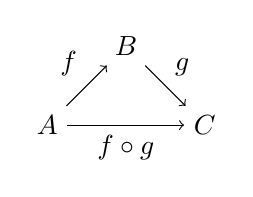
\begin{tikzpicture}
    \node (A) at (0,0) {$A$};
    \node (B) at (1,1) {$B$};
    \node (C) at (2,0) {$C$};

    \path[->]
    (A) edge node[above left] {$f$} (B)
    (B) edge node[above right] {$g$} (C)
    (A) edge node[below] {$f \circ g$} (C);
  \end{tikzpicture}
}

\section{Relationen}

\paragraph{Kartesisches Produkt}
\index{Kartesiches Produkt}
\index{Kreuzprodukt}

\begin{gather*}
  X_1 \times \cdots \times X_n := \{ (x_1, \cdots, x_n) \\
  | x_1 \in X_1, \cdots, x_n \in X_n \}
\end{gather*}

\index{Relation}
\paragraph{Relation $\mzSymbolEmph{\sim}$} von/auf $M$ nach $N$ ist Teilmenge $R \subseteq M \times N$. ($R' \subseteq N \times P$)

$$m \mzSymbolEmph{\sim} n \Leftrightarrow (m, n) \in R$$

\begin{description}
  \item [$\mzSymbolEmph{\equiv}$ Reflexiv]
        \index{Reflexivität}
        $\forall x \in M: (\mzMathEmph{x}, \mzMathEmph{x}) \in R$ \\
        $\Leftrightarrow \text{id}_M \subseteq R$
        % \\ $\not\Leftrightarrow \text{Irreflexiv} \land M \neq \emptyset$

  \item [Irreflexiv]
        \index{Irreflexivität}
        $\forall x \in M: (x, x) \mzSymbolEmph{\notin} R$ \\
        $\Leftrightarrow \text{id}_M \cap R = \emptyset$

  \item [$\mzSymbolEmph{\equiv}$ Sym.]
        \index{Symmetrie}
        $\forall (x,\mzMathEmph{y}) \in R: (\mzMathEmph{y}, x) \in R$ \\
        $\Leftrightarrow R \subseteq R^{-1}$

  \item [Antis.]
        \index{Antisymmetrie}
        $\forall x,y: ((x,y) \in R \land (y,x) \in R) \Rightarrow \mzMathEmph{x = y}$ \\
        $\Leftrightarrow R \cap R' \subseteq \text{id}_M$

  \item [$\mzSymbolEmph{\equiv}$ Transitiv]
        \index{Transitivität}
        $\forall \mzMathEmph{x},y,\mzMathEmph{z}: ((x,y) \in R \land (y,z) \in R) \Rightarrow (\mzMathEmph{x},\mzMathEmph{z}) \in R$ \\
        $\Leftrightarrow R;R \subseteq R$

  \item [Vollst.]
        \index{Vollständigkeit}
        $\forall \mzMathEmph{x},\mzMathEmph{y} \in M: (x,y) \in R \lor (y,x) \in R$ \\
        $\Leftrightarrow R \cup R^{-1} = M \times M$
\end{description}

% TODO: This <https://de.wikipedia.org/wiki/Relation_(Mathematik)#/media/Datei:Zusammenhang_der_Eigenschaften_bin%C3%A4rer_Relationen.svg>.

% ($\mzSymbolEmph{\equiv}$ Äquivalenzrelation)

% \mzScale{0.4}{
%   \begin{tikzpicture}
%     % X-Y-Axis
%     \draw[->] (-.5,0) -- (2,0) node[above] {$M$};
%     \draw[->] (0,-.25) -- (0,1) node[right] {$N$};
%     % Relation space.
%     \filldraw[fill=primary]
%     (0.8,0.45) circle[x radius=0.4, y radius=0.25] node {$R$};
%     % Label for Cartesian space.
%     \draw (2,1) node[left] {$M \times N$};
%   \end{tikzpicture}
% }

\subsection{Spezielle Relationen}

\begin{description}
  \item [Inverse Relation $R^{-1}$]
        \index{Inverse Relation}
        mit $R \in M \times N :=$ \\
        $\{ (n, m) \in N \times M \mid (m, n) \in R \}$

  \item [Komposition $R ; R$]
        \index{Komposition}
        mit $R' \in N \times P :=$ \\
        $\{ (m, p) \in M \times P \mid \exists n \in N: (m, n) \in R \land (n, p) \in R' \}$

  \item [Leere Relation $\emptyset$]
        \index{Leere Relation}

  \item [Identität $\text{id}_M$]
        \index{Relationsidentität}
        $:= \{ (m,m) \mid m \in M \}$ ($=$)

  \item [Allrelation $M \times M$]
        \index{Allrelation}

  \item [Äquivalenzrelation $\mzSymbolEmph{\equiv}$]
        \index{Äquivalenzrelation}
        reflexiv, symmetrisch und transitiv. (Gleichheit***)

        \item[Äquivalenzklasse $\mzMathEmph{[m]_\equiv}$]
        \index{Äquivalenzklasse}
        auf $M$, Vertreter $m \in M$.

        \begin{align*}
          [m]_\equiv & := \{ x \in M \mid m \equiv x \}        \\
                     & \Leftrightarrow [m]_\equiv = [x]_\equiv
        \end{align*}

  \item [Zerlegung $\mzSymbolEmph{\mathcal{N}}$]
        \index{Zerlegung}
        $\subseteq \mathcal{P}(M)$ von $M$.

        \begin{itemize}
          \item $\emptyset \notin \mathcal{N}$
          \item $M = \bigcup \mathcal{N}$
          \item $N \cap N' = \emptyset$ \\
                ($N, N' \in \mathcal{N}: N \neq N'$)
          \item (Korrespondiert zur ÄR.)
        \end{itemize}

  \item [Quotient $\mzMathEmph{(M / \equiv)}$]
        \index{Mengenquotient}
        Sei $\equiv$ ÄR. auf $M$. (ist Zerlegung)

        $$(M / \equiv) := \{ [m]_\equiv \mid m \in M \}$$
\end{description}